\documentclass[letterpaper,12pt]{article}

\usepackage{threeparttable}
\usepackage{geometry}
\geometry{letterpaper,tmargin=1in,bmargin=1in,lmargin=1.25in,rmargin=1.25in}
\usepackage[format=hang,font=normalsize,labelfont=bf]{caption}
\usepackage{amsmath}
\usepackage{multirow}
\usepackage{array}
\usepackage{delarray}
\usepackage{amssymb}
\usepackage{amsthm}
\usepackage{lscape}
\usepackage{natbib}
\usepackage{setspace}
\usepackage{float,color}
\usepackage[pdftex]{graphicx}
\usepackage{mathrsfs}  
\usepackage{pdfsync}
\usepackage{verbatim}
\usepackage{placeins} \usepackage{geometry}
\usepackage{pdflscape}
\synctex=1
\usepackage{hyperref}
\hypersetup{colorlinks,linkcolor=red,urlcolor=blue,citecolor=red}
\usepackage{bm}
\usepackage{amssymb}
\usepackage{listings}


\theoremstyle{definition}
\newtheorem{theorem}{Theorem}
\newtheorem{acknowledgement}[theorem]{Acknowledgement}
\newtheorem{algorithm}[theorem]{Algorithm}
\newtheorem{axiom}[theorem]{Axiom}
\newtheorem{case}[theorem]{Case}
\newtheorem{claim}[theorem]{Claim}
\newtheorem{conclusion}[theorem]{Conclusion}
\newtheorem{condition}[theorem]{Condition}
\newtheorem{conjecture}[theorem]{Conjecture}
\newtheorem{corollary}[theorem]{Corollary}
\newtheorem{criterion}[theorem]{Criterion}
\newtheorem{definition}{Definition} % Number definitions on their own
\newtheorem{derivation}{Derivation} % Number derivations on their own
\newtheorem{example}[theorem]{Example}
\newtheorem*{exercise}{Exercise} % Number exercises on their own
\newtheorem{lemma}[theorem]{Lemma}
\newtheorem{notation}[theorem]{Notation}
\newtheorem{problem}[theorem]{Problem}
\newtheorem{proposition}{Proposition} % Number propositions on their own
\newtheorem{remark}[theorem]{Remark}
\newtheorem{solution}[theorem]{Solution}
\newtheorem{summary}[theorem]{Summary}
\bibliographystyle{aer}
\newcommand\ve{\varepsilon}
\renewcommand\theenumi{\roman{enumi}}

\title{Math Sec 3.6}
\author{Rex McArthur\\Math 320}


\begin{document}
\maketitle

\exercise{3.33}\\
We will begin by using Markov's inequality, and find
\begin{align*}
    P \left( \left| \frac{B}{n} - p \right| \geq \varepsilon \right) &= P \left( \left| \frac{B}{n} - p \right|^2 \geq \varepsilon^2 \right) \\ 
    P \left( \left| \frac{B}{n} - p \right|^2 \geq \varepsilon^2 \right) &\leq  \frac{E \left[ \left( \frac{B}{n} - p \right)^2 \right]}{\varepsilon^2} \\
    &= \frac{E \left[ \left( \frac{B-pn}{n} \right)^2 \right]}{\varepsilon^2} \\
    &= \frac{E \left[ \left( B-pn \right)^2 \right]}{n^2 \varepsilon^2} \\
\end{align*}
\begin{align*}
    &= \frac{E \left[ B^2 \right]-E\left[   2Bnp  \right] + E\left[(np)^2  \right]}{n^2 \varepsilon^2} \\
    &= \frac{E \left[ B^2 \right]-2npE\left[   B  \right] + E\left[(np)^2  \right]}{n^2 \varepsilon^2} \\
\end{align*}
\begin{align*}
    &= \frac{E \left[ B^2 \right]-2E\left[   B  \right]^2 + E\left[B  \right]^2}{n^2 \varepsilon^2} \\
    &= \frac{E \left[ B^2 \right]-E\left[   B  \right]^2 }{n^2 \varepsilon^2} \\
    &= \frac{\sigma_B^2}{n^2 \varepsilon^2} \\
\end{align*}
    $B$ is a binomial distributed random variable, thus, we can say, 
\begin{align*}
    &= \frac{p(1-p)}{n^2 \varepsilon^2} \\
\end{align*}
   Note, $n \geq 1$ 
\begin{align*}
    &\leq \frac{p(1-p)}{n \varepsilon^2} \\
\end{align*}

\exercise{3.34}\\

Note,
\[P \left( \Big| \frac{1}{n} \sum^{n}_{i=1} X_i \Big| < \varepsilon \right) = 
P \left( \Big| \frac{X_1 + X_2 +\cdots+ X_n}{n} - 0 \Big| < \varepsilon\right) = 
P \left( \Big| \frac{X_1 + X_2 +\cdots+ X_n}{n} - \mu \Big| < \varepsilon\right)\]
Is the complement of the law of large numbers equation given to us. Thus we know that this equation summed with the Weak Law of Large Numbers will equal 1, and because the weak Large of Numbers half will tend to zero as n gets large, we know the other half must equal, or:
\[P \left( \Big| \frac{X_1 + X_2 +\cdots+ X_n}{n} - \mu + 0 \Big| < \varepsilon\right) = 1\]

\exercise{3.35}\\
For a random variable, $X_i$, we have by the Central limit Theorem,
\begin{align*}
    P( \sum^{n}_{i=1} X_i \leq 2000) &= P( \sum^{n}_{i=1}\frac{ X_i - n\mu }{\sqrt{n} \sigma}\leq \frac{ 2000 }{\sqrt{n} \sigma}) \\
    &= P( \sum^{n}_{i=1}\frac{ X_i - 10\cdot176 }{\sqrt{10} \cdot 30}\leq \frac{240}{\sqrt{10} \cdot 30}) \\
    &= P( \sum^{n}_{i=1}\frac{ X_i - 1760 }{\sqrt{10} \cdot 30}\leq \frac{240}{\sqrt{10} \cdot 30}) \\
\end{align*}
Which corresponds to the integral
\[\frac{1}{\sqrt{2 \pi}} \int_{-\infty}^{\frac{240}{\sqrt{10}\cdot 30}} e^{-x^2/2} dx\] 
Which is $\approx .99429$ calculated using a computer.


\exercise{3.36}\\
Following a similar precedure as above, we find that for a random variable, $X_i$, we have by the Central limit Theorem,
\begin{align*}
    P( \sum^{n}_{i=1} X_i \geq 5500) &= 1 - P( \sum^{n}_{i=1}\frac{ X_i - 6242\cdot.801 }{\sqrt{6242} \cdot.399428}\leq \frac{5500- 6242\cdot.801 }{\sqrt{6242}\cdot .399428}) \\
    &=1 -  P( \sum^{n}_{i=1}\frac{ X_i - 5000 }{\sqrt{6242}\cdot .399428}\leq \frac{500}{\sqrt{6242} \cdot.399428}) \\
\end{align*}
Which corresponds to the integral
\[1 - \frac{1}{\sqrt{2 \pi}} \int_{-\infty}^{\frac{500}{\sqrt{6242}\cdot .399428}} e^{-x^2/2} dx\]
Which is $\approx 2.22045\times10^{-16}$, or a $really$ small number.

\exercise{3.37}\\
Let,
\[X_i = 
\begin{cases}
    1 & \text{if dice roll is  6 }\\
    0 & \text{ else}\\
\end{cases}
\]
The probability of $X_i$ is $\frac{1}{6}$ with variance $\frac{\sqrt{5}}{6}$, Thus, we can apply the Central Limit Theoreom.

\begin{align*}
    P\left( 150 \leq \sum^{n}_{i=1} X_i \leq 200 \right) &= P\left( \frac{150 - \frac{1}{6}900}{6\sqrt{900}\sqrt{5}} \leq \sum^{n}_{i=1} \frac{X_i - \frac{1}{6}900}{6\sqrt{900}\sqrt{5}} \leq \frac{200-\frac{1}{6}900}{6\sqrt{900}\sqrt{5}} \right) \\
    &= P\left( 0 \leq \sum^{n}_{i=1} \frac{X_i - 150}{5\sqrt{5}} \leq \frac{50}{5\sqrt{5}} \right) \\
\end{align*}
Which gives us, 
\[ \frac{1}{\sqrt{2 \pi}} \int_{0}^{\frac{50}{5\sqrt{5}}} e^{-x^2/2}dx\]
Which is $\approx .499996$

\exercise{3.38}\\
\begin{lstlisting}
"""
Author: Rex McArthur
Date: Oct. 25, 2015
"""
import numpy as np
from scipy import stats
import matplotlib.pyplot as plt
import matplotlib.mlab as mlab
import sys

def exercise_38(a,b):
    '''
    Calculates and plots the different values on the same plot,
    using matplotlib and various stats modules from scipy
    Calclculates using values [1, 2, 4, 8, 16, 32]
    Also, plots the histograms normed
    '''
    mean, var = stats.beta.stats(a,b, moments='mv')
    vec = np.linspace(stats.beta.ppf(.01,a,b), stats.beta.ppf(.99, a, b), 100)
    plt.plot(vec,stats.beta.pdf(vec,a,b))
    print "Mean: ", mean
    print "Variance", var
    n_val = np.array([1, 2, 4, 8, 16, 32])

    for i in n_val:
        plt.plot(vec,mlab.normpdf(vec,mean,np.sqrt(var/i)))
        xbar = np.average(stats.beta.rvs(a,b,size=(i,1000)),axis = 0)
        plt.hist(xbar,normed=True)
    plt.show()

exercise_38(1,4)
exercise_38(1,1)

\end{lstlisting}
Mean:  0.2\\
Variance:  0.026666667\\
\[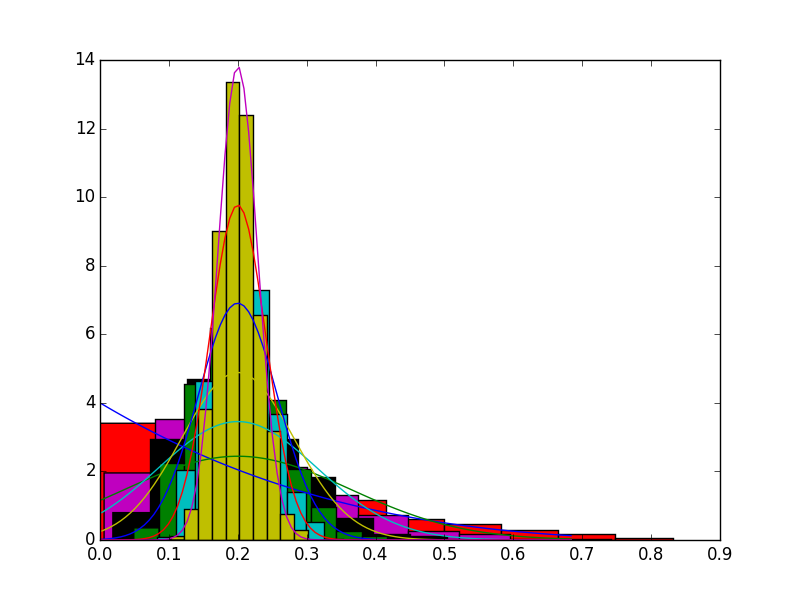
\includegraphics[scale = .7]{figure_1.png}\]

Mean:  0.5\\
Variance:  0.08333333333\\
\[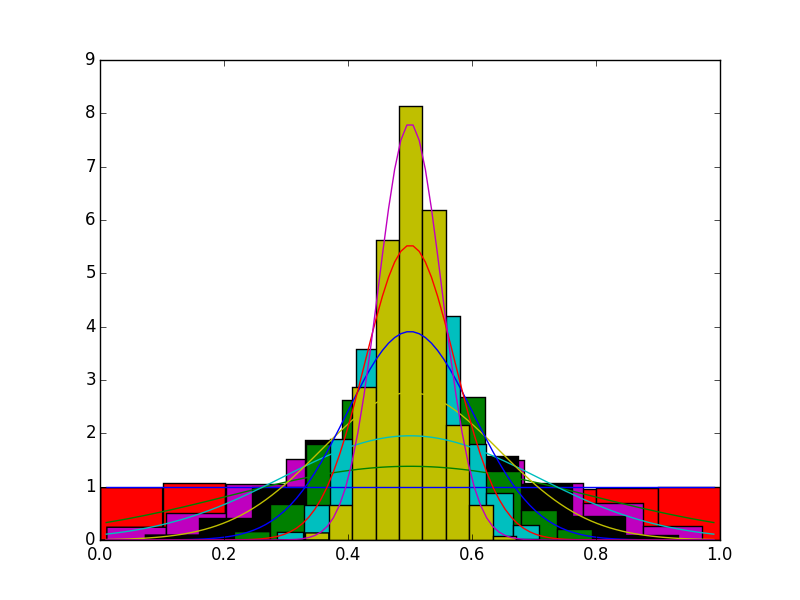
\includegraphics[scale = .7]{figure_2.png}\]


\end{document}
